<<<<<<< HEAD
\chapter{Математический аппарат квантовой механики}

\begin{sloppypar}
  \section{Состояние и волновая функция. Принцип суперпозиции состояний. Дираковская формулировка квантовой механики. Вектор состояния.}
\end{sloppypar}

1938 г. -- символика Дирака для описания состояний

$\ket{\cdots}$ -- вектор состояний

$\ket{\vr}$, $\ket{\vp}$, $\ket{E}$, $\ket{nlm_l}$

Сформулируем \textbf{принцип суперпозиции состояний}:
\begin{stmt}
Если квантовая система может находиться в состояниях, описываемых волновыми функциями $\psi_1$ и $\psi_2$, то она может находиться и в состоянии $\psi$, описываемой их линейной комбинацией:
$$
\psi = c_1 \psi_1 + c_2 \psi_2, ~~ \text{~где~} c_1, c_2 \in \mathbb{C}
$$
$c_1, c_2$ - произвольные (с точностью до условия нормировки) комплексные числа.
\end{stmt}

\begin{figure}[here]
  \centering
  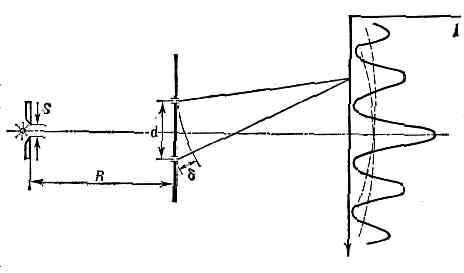
\includegraphics[scale=0.4]{figs/3_1}
  \label{fig:3_1}
\end{figure}

$$
\lambdabar_{\text{д.б.}} = \frac{\hbar}{p} \lesssim d
$$

\begin{equation}
\label{eq:3_1_1}
\Psi(\vr, t) = \brs{\psi_{1}(\vr_1) + \psi_{2}(\vr_2)} e^{-i E t /\hbar}
\end{equation}

$$
\frac{E}{\hbar} = \omega
$$

\begin{equation}
\label{eq:3_1_2}
\begin{gathered}
\abs{\Psi(\vr, t)}^2 = \abs{\psi_1(\vr_1) + \psi_2(\vr_2)}^2 = \abs{\psi_1}^2 + \abs{\psi_2}^2 + \underbrace{(\psi_1^* \psi_2 + \psi_1 \psi_2^*)}_{2 \Re(\psi_1 \psi_2^*)} = \\ = \abs{\psi_1}^2 + \abs{\psi_2}^2 + 2\abs{\psi_1}\abs{\psi_2} \cos{(\phi_1 - \phi_2)}
\end{gathered}
\end{equation}

$$
\Delta \phi = \phi_1 - \phi_2 ~~~~~~ \abs{\psi_1} = \abs{\psi_2}
$$

\begin{equation}
\label{eq:3_1_3}
\abs{\Psi}^2 = 4 \abs{\psi_1}^2 \cos^2{\frac{\Delta \phi}{2}}
\end{equation}

При этом $\abs{\Psi}^2_{max} = 4 \abs{\psi_1}^2$

Свойство \textbf{линейности} пространства состояний:
\begin{equation}
\label{eq:3_1_4}
\ket{\psi} = c_1\ket{\psi_1} + c_2\ket{\psi_2}, ~~\text{~где~} c_1, c_2 \in  \mathbb{C}
\end{equation}

\begin{stmt}[Первый постулат квантовой механики]
Квантовое состояние системы полностьб определяется вектором состояния $\ket{\psi}$. Векторы $\ket{\psi}$ и $c\ket{\psi} ~(c \neq 0)$ определяют одно и то же состояние.
\end{stmt}

Свойства пространства состояний:
\begin{enumerate}
\item $\ket{\psi} + \ket{\phi} = \ket{\phi} + \ket{\psi}$ (аксиома коммутативности)
\item $\brs{\ket{\psi} + \ket{\phi}} + \ket{\chi} = \ket{\psi} + \brs{\ket{\phi} + \ket{\chi}}$ (аксиома ассоциативности)
\item $c\brc{\ket{\phi} + \ket{\psi}} = c\ket{\phi} + c\ket{\psi}$ (аксиома дистрибутивности)
\item $(c_1 + c_2)\ket{\psi} = c_1\ket{\psi} + c_2\ket{\psi}$ (аксиома дистрибутивности)
\item $0 \cdot \ket{\psi} \equiv \ket{0} = 0$ (отсутствие квантового объекта)
\end{enumerate}

Векторное пространство состояний наделено скалярным произведением:
$$
\bk{\phi}{\psi} \in \mathbb{C}
$$

\begin{defn}
Пусть $\vec{q} = (q_1, ..., q_n)$ -- конфигурационное пространство. Тогда скалярное произведение определяется следующим образом:
\begin{equation}
\label{eq:3_1_5}
\bk{\phi}{\psi} = \int \phi^*\underbrace{(q_1, ..., q_n)}_{\vec{q}} \psi\underbrace{(q_1, ..., q_n)}_{\vec{q}} \underbrace{d q_1 ... d q_n}_{d\vec{q}}
\end{equation}
\end{defn}

Если $\bk{\phi}{\psi} = 0$, то $\phi$ и $\psi$ \textbf{взаимно ортогональны}.

Свойства скалярного произведения:
\begin{enumerate}
\item Из \eqref{eq:3_1_5}: $\bk{\phi}{\psi} = \bk{\psi}{\phi}^*$
\item Если $\ket{\tilde{\phi}} = \lambda_1\ket{\phi}$ и $\ket{\tilde{\psi}} = \lambda_2\ket{\psi}$, то $\bk{\tilde{\phi}}{\tilde{\psi}} = \lambda_1^* \lambda_2 \bk{\phi}{\psi}$
\item
	\begin{itemize}
		\item $\bk{\psi}{\psi} \geqslant 0$
		\item $\bk{\psi}{\psi} = 0 ~\Leftrightarrow~ \ket{\psi} = 0$
		\item $\norm{\psi} = \sqrt{\bk{\psi}{\psi}}$
	\end{itemize}
\end{enumerate}

Пространство состояний линейное, на нем определено скалярное произведение, и оно обладает свойством полноты, а значит является \textbf{пространством Гильберта} (обозначается буквой $\mathbb{H}$)

$\ket{\psi}$ можно понимать как столбец: $\vec{\psi} = \left(\begin{array}{c} \psi_1 \\ \psi_2 \end{array}\right)$

$$
\bk{\phi}{\psi} = (\phi_1^*, \phi_2^*) \left(\begin{array}{c} \psi_1 \\ \psi_2 \end{array}\right) = \phi_1^*\psi_1 + \phi_2^* \psi_2
$$

Т.е. состоянию $\ket{\psi}$ соответствует элемент дуального (сопряжённого) по отношению к $\mathbb{H}$ пространства $\mathbb{H}^*$, обозначаемый как $\bra{\psi}$ (или в виде строки: $(\psi_1^*, \psi_2^*)$).

Сопряжённые состояния связаны операцией \textbf{эрмитового сопряжения}, обозначаемой символом $^\dag$. На матричном языке эта операция состоит в выполнении транспонирования и комплексного сопряжения.
$$
\bra{\psi} = \ket{\psi}^\dag
$$

$$
\forall \ket{\psi} \in \mathbb{H}~~ \exists \bra{\phi} \in \mathbb{H}^* : \bk{\phi}{\psi} \in \mathbb{C}
$$

\noindent
$\ket{\psi}$ -- \textbf{кет-вектор} \\
$\bra{\psi}$ -- \textbf{бра-вектор}

Из \eqref{eq:3_1_4}:
$$
\begin{gathered}
\ket{\psi} = c_1 \ket{\psi_1} + c_2 \ket{\psi_2} \\
\bra{\psi} = c_1^* \bra{\psi_1} + c_2^* \bra{\psi_2}
\end{gathered}
$$

Нормировка:
$$
\begin{gathered}
\bk{\psi}{\psi} = \bk{\psi_1}{\psi_1} = \bk{\psi_2}{\psi_2} = 1 \\
\bk{\psi}{\psi} = \abs{c_1}^2 + \abs{c_2}^2 + 2 \Re{c_1^* c_2 \bk{\psi_1}{\psi_2}} = 1
\end{gathered}
$$

Если $\bk{\psi_1}{\psi_2} = 0$ (ортогональные состояния), то $\abs{c_1}^2 + \abs{c_2}^2 = 1$.

Вероятностная интерпретация: $\abs{c_1}^2$ ($\abs{c_2}^2$) -- вероятность обнаружить систему в состоянии \circled{1} (в состоянии \circled{2})

\begin{stmt}[Второй постулат квантовой механики]
Если измерение в состоянии \circled{1} даёт результат \circled{1}, а измерение в состоянии \circled{2} даёт результат \circled{2}, то измерение в суперпозиции этих состояний даёт либо результат \circled{1}, либо результат \circled{2}.
\end{stmt}

\section{Наблюдаемые и операторы физических величин. Линейные и эрмитовые операторы}

$F$ -- физическая (или, в терминологии Дирака, \textbf{наблюдаемая}) величина.

$F$ соответствует $\op{F}$:

$$
\begin{gathered}
\op{F}: D_{\op{F}} \to R_{\op{F}} \\
\ket{\phi} = \op{F} \ket{\psi} \in R_{\op{F}}, ~~\text{где}~~ \ket{\phi} \in D_{\op{F}}
\end{gathered}
$$

\begin{defn}
Оператор $\op{F}$ называется \textbf{линейным}, если для него выполняется:
\begin{equation}
\label{eq:3_2_1}
	\begin{gathered}
	\op{F}(c_1 \ket{\psi_1} + c_2 \ket{\psi_2}) = c_1 \op{F}\ket{\psi_1} + c_2 \op{F}\ket{\psi_2}, \\
	\text{где}~ \ket{\psi_1}, \ket{\psi_2} \in D_{\op{F}}~;~ c_1, c_2 \in \mathbb{C}\\
	\end{gathered}
\end{equation}
В этом случае:\footnote{проверить определение, просто на всякий случай}
$$
c_1 \ket{\psi_1} + c_2\ket{\psi_2} \xrightarrow{~~\op{F}~~} c_1 \ket{\phi_1} + c_2 \ket{\phi_2}
$$
\end{defn}

Алгебра линейных операторов:
\begin{enumerate}
\item Умножение на комплексное число:
$$
(c\op{F}) \ket{\psi} \equiv \underbrace{\left. c (\op{F} \ket{\psi}) \right|_{\text{\eqref{eq:3_2_1}}} = \op{F} (c \ket{\psi})}_{\text{свойство однородности $\op{F}$}}
$$
\item Коммутативность операции сложения:
$$
\begin{gathered}
(\op{F} + \op{G})\ket{\psi} \equiv \left. \op{F}\ket{\psi} + \op{G}\ket{\psi} \right|_{\text{из 1.}} = \op{G}\ket{\psi} + \op{F}\ket{\psi} = (\op{G} + \op{F})\ket{\psi}
\Rightarrow~ \op{F} + \op{G} = \op{G} + \op{F}
\end{gathered}
$$
\item Произведение операторов:
$$
\begin{gathered}
\op{P} = \op{F}\op{G} ~~\Rightarrow~~ \op{P}\ket{\psi} = \op{F}(\op{G}\ket{\psi})
\end{gathered}
$$
В общем случае операция произведения некоммутативна: $\op{F}\op{G}\ket{\psi} \neq \op{G}\op{F}\ket{\psi}$
\end{enumerate}

\begin{defn}
Выражение $\op{F}\op{G} - \op{G}\op{F}$ называется \textbf{коммутатором} операторов $\op{F}$ и $\op{G}$ и обозначается квадратными скобками:
\begin{equation}
\label{eq:3_2_2}
\brs{\op{F}, \op{G}} \equiv \op{F}\op{G} - \op{G}\op{F}
\end{equation}
Говорят, что операторы \textbf{коммутируют}, если $\brs{\op{F}, \op{G}} = 0$.
\end{defn}

Свойства коммутаторов:
\begin{enumerate}
\item Любой оператор коммутирует с константой:
$$
\brs{\op{F}, c} = 0,~~ c = \const
$$
\item Если между двумя пространствами состояний есть взаимно-однозначное соответствие, т.е.:
$$
\ket{\phi} = \op{F}\ket{\psi} ~~\to~~ \ket{\psi} = \op{G}\ket{\phi}
$$
то $\op{F}$ и $\op{G}$ являются \textbf{обратными друг к другу операторами}:
\begin{equation}
\label{eq:3_2_3}
\op{F}\op{G} = \op{G}\op{F} = 1
\end{equation}
Оператор, обратный к данному обозначается $\op{F}^{-1}$.
\end{enumerate}

\begin{equation}
\label{eq:3_2_3_add}
\op{F}\op{F}^{-1} = \op{F}^{-1}\op{F} = 1
\tag{\ref{eq:3_2_3}$'$}
\end{equation}

Обратный оператор произведения:
\begin{equation}
\label{eq:3_2_4}
(\op{F}\op{G})^{-1} = \op{G}^{-1} \op{F}^{-1}
\end{equation}

\begin{excr}
Доказать \eqref{eq:3_2_4}, используя \eqref{eq:3_2_3_add}.
\end{excr}

Рассмотрим действие $\op{F}$ в гильбертовом пространстве $\mathbb{H}$ (и, соответственно, оператора $\op{F}^\dag$ в $\mathbb{H}^*$):

$$
\ket{\chi} = \op{F}\ket{\psi} ~\to~ \ket{\chi}^\dag = \left. (\op{F}\ket{\psi})^\dag \right|_{(\op{A}\op{B})^\dag = \op{B}^\dag \op{A}^\dag} = \bra{\psi} \op{F}^\dag
$$

\begin{equation}
\label{eq:3_2_5}
\boxed{
	\bra{\chi} = \bra{\psi} \op{F}^\dag
}
\end{equation}

Из \eqref{eq:3_2_5}:
$$
\bk{\chi}{\phi} = \bfk{\psi}{\op{F}^\dag}{\phi} = \bk{\phi}{\chi}^* = \bfk{\phi}{\op{F}}{\psi}^*
$$

\begin{defn}
Эрмитово-сопряжённым к $\op{F}$ называется следующий оператор:
\begin{equation}
\label{eq:3_2_6}
\boxed{
	\bfk{\psi}{\op{F}^\dag}{\phi} = \bfk{\phi}{\op{F}}{\psi}^*
}
\end{equation}
\end{defn}

Свойства эрмитово-сопряжённых операторов:
\begin{itemize}
\item $(c\op{F})^\dag = c^* \op{F}^\dag$
\item $(\op{F}^\dag)^\dag = \op{F}$
\item $(\op{F} + \op{G})^\dag = \op{F}^\dag + \op{G}^\dag$
\item $(\op{F}\op{G})^\dag = \op{G}^\dag \op{F}^\dag$
\end{itemize}

\begin{excr}
Доказать приведённые выше свойства.
\end{excr}

\begin{defn}
Если $\op{F}^\dag = \op{F}$ или выполняется следующее равенство:
\begin{equation}
\label{eq:3_2_7}
\forall \ket{\psi},\ket{\phi} \in D_{\op{F}} ~~\to~~  \bk{\psi}{\op{F}\psi} = \bfk{\phi}{\op{F}}{\psi}^*
\end{equation}
то оператор $\op{F}$ называется \textbf{эрмитовым} или \textbf{самосопряжённым}.
\end{defn}

Для состояний $\ket{\psi}$ и $\ket{\phi}$:
$$
\op{F}\ket{\psi} \equiv \ket{\op{F}\psi}
$$

Альтернативное определение эрмитового сопряжения: $\op{F}^\dag$ эрмитово-сопряжённый, если:
\begin{equation}
\label{eq:3_2_6_add}
\boxed{
	\bk{\phi}{\op{F}\psi} = \bk{\op{F}^\dag\phi}{\psi}
} = \bk{\psi}{\op{F}^\dag \phi}^*
\tag{\ref{eq:3_2_6}$'$}
\end{equation}
или
\begin{equation}
\label{eq:3_2_6_add_x2}
\boxed{
	\bk{\psi}{\op{F}^\dag \phi} = \bk{\op{F} \psi}{\phi}
}
\tag{\ref{eq:3_2_6}$''$}
\end{equation}
что эквивалентно:
$$
\int \psi^*(\vec{q}) \op{F}^\dag \phi(\vec{q}) d\vec{q} = \int \brc{\op{F} \psi(\vec{q})}^* \phi(\vec{q}) d\vec{q}
$$

\begin{defn}
$\op{F}$ называется \textbf{эрмитовым} (самосопряжённым), если $\op{F}^\dag = \op{F}$, т.е.:
\begin{equation}
\label{eq:3_2_7_add}
\forall \ket{\psi}, \ket{\phi} \in D_{\op{F}}  ~\to~ \boxed{ \bk{\psi}{\op{F} \phi} = \bk{\op{F}\psi}{\phi} }
\tag{\ref{eq:3_2_7}$'$}
\end{equation}
или
$$
\int \psi^*(\vec{q}) \op{F} \phi(\vec{q}) d\vec{q} = \int \brc{\op{F} \psi(\vec{q})}^* \phi(\vec{q}) d\vec{q}
$$
\end{defn}

Замечание:
\begin{enumerate}
\item $\norm{\psi} < \infty$, $\norm{\phi} < \infty$
\item $\norm{\op{F} \psi} < \infty$, $\norm{\op{F} \phi} < \infty$
\end{enumerate}

\begin{defn}
Выражение:
$$
\bk{\phi}{\op{F}\psi} \equiv \bfk{\phi}{\op{F}}{\psi} = \int \phi^*(\vec{q})\op{F}\psi(\vec{q}) d\vec{q}
$$
называется \textbf{матричным элементом} оператора $\op{F}$ на функциях $\phi$ и $\psi$, или матричным элементом $\op{F}$ \textbf{в обкладках} $\bra{\phi}$ и $\ket{\psi}$  

Величина $\bk{\psi}{\op{F}\psi} \equiv \bfk{\psi}{\op{F}}{\psi}$ называется \textbf{диагональным матричным элементом}.
\end{defn}

Из \eqref{eq:2_2_1}, среднее значение физической величины:
\begin{equation}
\label{eq:3_2_8}
\boxed {
	\avg{F} = \bk{\psi}{\op{F}\psi} = \bfk{\psi}{\op{F}}{\psi}
}
\end{equation}

Для величины, принимающей действительные значения, $\avg{F} = \avg{F}^*$.

Из \eqref{eq:3_2_8}:
\begin{equation}
\label{eq:3_2_9}
\bfk{\psi}{\op{F}}{\psi} = \left .\bfk{\psi}{\op{F}}{\psi}^* \right|_{\text{\eqref{eq:3_2_6}}} = \bfk{\psi}{\op{F}^\dag}{\psi}
\end{equation}

Следовательно: $\op{F} = \op{F}^\dag$.

Таким образом, физическим (наблюдаемым) величинам соответствуют \textbf{эрмитовы операторы}.

Рассмотрим среднеквадратичное отклонение (дисперсию):
\begin{equation}
\label{eq:3_2_10}
\avg{(\Delta F)^2} \equiv \avg{(F - \avg{F}^2)}
\end{equation}

Из \eqref{eq:2_2_1}:
\begin{equation}
\label{eq:3_2_11}
\avg{(\Delta F)^2} = \bfk{\psi}{(\op{F} - \avg{F})^2}{\psi}
\end{equation}

Заметим, что $\op{F} - \avg{F}$ -- эрмитов оператор.

\begin{equation}
\label{eq:3_2_12}
\left. \avg{(\Delta F)^2} \right|_{\text{\eqref{eq:3_2_7_add}}} = \bk{(F - \avg{F})\psi}{(F - \avg{F})\psi} = \int \abs{\brc{F - \avg{F}}\psi}^2 d\vec{q} \geqslant 0
\end{equation}

Если $\avg{(\Delta F)^2} = 0$, т.е. величина не имеет разброса, то из \S 3 гл. 2:
\begin{equation}
\label{eq:3_2_13}
\op{F}\ket{\psi} = \avg{F}\ket{\psi}
\end{equation}

Примем $\avg{F} = f$ -- собственное значение оператора $\op{F}$.

Можно переписать формулу \eqref{eq:2_3_2}:
\begin{equation}
\label{eq:3_2_14}
\op{F}\ket{\psi_{f}} = f \ket{\psi_{f}}
\end{equation}

\begin{stmt}[Третий постулат квантовой механики]
Физическая величина $F$ в любом квантовом состоянии может принимать только те значения, которые принадлежат спектру её оператора $\op{F}$.
\end{stmt}

\begin{thm}
Если оператор $\op{F}$ эрмитов, то он имеет вещественные собственные значения.
\end{thm}
\begin{proof}
Левая часть \eqref{eq:3_2_14}:
$$
\left. \bfk{\psi_f}{\op{F}}{\psi_f}^* \right|_{\text{\eqref{eq:3_2_7}}} = \bfk{\psi_f}{\op{F}}{\psi_f}
$$
Правая часть \eqref{eq:3_2_14}:
$$
f^*\bk{\psi_f}{\psi_f}^* = f^* \bk{\psi_f}{\psi_f} = f\bk{\psi_f}{\psi_f}
$$
Следовательно $\boxed{f^* = f}$.
\end{proof}

\begin{stmt}
Эрмитовы операторы изображают вещественные (наблюдаемые) величины.
\end{stmt}

\section{Условие ортогональности и полноты для собственных функций операторов физических величин}

Уравнение \eqref{eq:2_3_3} на собственные значения $\op{F}$ в векторном виде:

\begin{equation}
\label{eq:3_3_1}
\op{F}\ket{\psi_n} = f_n \ket{\psi_n} ~~\text{или}~~ \op{F}\ket{n} = f_n\ket{n}
\end{equation}
где $\psi_n \equiv \ket{n}$, $n = 0, 1, 2, ...$

\noindent
$f_n \to \ket{\psi_n}$ -- невырожденный (простой) спектр\\
$f_n \to \brcr{\ket{\psi_n^{(1)}}, \ket{\psi_n^{(2)}}, ..., \ket{\psi_n^{(g)}} }$ -- вырожденный спектр

\begin{defn}
Максимальное количество линейно-независимых собственных векторов (собственных функций), отвечающих данному собственному значению, называется \textbf{кратностью вырождения} этого собственного значения.
\end{defn}

\begin{stmt}
Собственные векторы эрмитового оператора, соответствующие различным собственные значениям, взаимно ортогональны.
\end{stmt}
\begin{proof}

\begin{equation}
\label{eq:3_3_2}
	\begin{gathered}
		\bra{\psi_m}: \op{F}\ket{\psi_n} = f_n \ket{\psi_n} \\
		\bra{\psi_n}: \op{F}\ket{\psi_m} = f_m \ket{\psi_m} \\
		f_n \neq f_m
	\end{gathered}
\end{equation}

$$
\left. \bfk{\psi_m}{\op{F}}{\psi_n} - \bfk{\psi_n}{\op{F}}{\psi_m}^\dag \right|_{\text{\eqref{eq:3_2_7}}} = 0 = f_n \bk{\psi_m}{\psi_n} - \underbrace{f_m^*}_{= f_m} \bk{\psi_n}{\psi_m}^*
$$

\begin{equation}
\label{eq:3_3_3}
(f_n - f_m) \bk{\psi_m}{\psi_n} = 0
\end{equation}

$f_m \neq f_n ~~\to~~ \boxed{\bk{\psi_m}{\psi_n} = 0}$

\end{proof}

\begin{equation}
\label{eq:3_3_4}
\bk{\psi_n}{\psi_n} = 1
\end{equation}

Из \eqref{eq:3_3_3} и \eqref{eq:3_3_4} получим условие ортонормированности:
\begin{equation}
\label{eq:3_3_5}
\boxed{
	\bk{\psi_m}{\psi_n} = \bk{m}{n} = \delta_{mn}
}
\end{equation}

$$
f_n ~\to~ \brcr{\ket{\psi_n^{(i)}}} ~~ i = \overline{1,g}
$$

\begin{equation}
\label{eq:3_3_6}
f_n ~\to~ \ket{\psi_n^s} = \sum_{i=1}^{g} c_i^{(s)} \ket{\psi_n^{(i)}}
\end{equation}

Посредством ортогонализации методом Грамма-Шмидта, коэффициенты $c_i^{(s)}$ возможно подобрать так, что $\bk{\psi_n^{(t)}}{\psi_n^{(s)}} = \delta_{ts}$

Ортонормированная система -- базис в гильбертовом пространстве состояний.

\begin{equation}
\label{eq:3_3_7}
\forall \ket{\psi} \in \mathbb{H} ~~~ \op{F}:~~ \ket{\psi} = \sum_n c_n \ket{\psi_n}
\end{equation}

$$
\bk{\psi_m}{\psi} = \sum_n c_n \underbrace{\bk{\psi_m}{\psi_n}}_{=\delta{mn}~(\text{из \eqref{eq:3_3_5}})} = \sum_n c_n \delta_{mn} = c_m
$$

$c_n = \bk{\psi_n}{\psi}$ -- коэффициенты -- проеции вектора на соответствеющие орты.

Для векторов-состояний $\ket{\psi}$ и $\bra{\phi}$ выполняется $\bk{\phi}{\psi} \in \mathbb{C}$

\begin{equation}
\label{eq:3_3_8}
\op{P}_{\psi} = \proj{\psi}{\phi}
\end{equation}

\begin{equation}
\label{eq:3_3_9}
\op{P}_\psi \ket{\chi} = \ket{\psi} \underbrace{\bk{\phi}{\chi}}_{= c} = c \ket{\psi}
\end{equation}

Следовательно, $\op{P}_\psi$ -- \textbf{оператор проектирования}.

Из \eqref{eq:3_3_7}:
\begin{equation}
\label{eq:3_3_10}
\ket{\psi} = \sum_n \ket{\psi_n} \bk{\psi_n}{\psi} = \brc{\sum_n \proj{\psi_n}{\psi_n}} \ket{\psi}
\end{equation}

Итого, получаем \textbf{условие полноты} (операторное разложение единицы) системы собственных векторов оператор $\op{F}$:
\begin{equation}
\label{eq:3_3_11}
\boxed {
	\sum_n \proj{\psi_n}{\psi_n} = \mathds{1}
}
\end{equation}

\begin{equation}
\label{eq:3_3_12}
\ket{\psi_n} \underbrace{\bk{\psi_n}{\psi}}_{ = c_n} \equiv \op{P}_n \ket{\psi} = c_n \ket{\psi_n}
\end{equation}
где $\proj{\psi_n}{\psi_n} = \op{P}_n$ -- проектор на n-е базисное состояние.

\noindent
Свойства проекторов:
\begin{enumerate}
\item $\op{P}_n$ -- эрмитов
\item $\op{P}_n^2 = \op{P}_n$
\item собственные значения $\op{P}_n$: $\lambda = \brcr{0, 1}$
\end{enumerate}
\begin{excr}
Доказать вышеперечисленные свойства.
\end{excr}

$$
\begin{gathered}
\left. \ket{\psi} \right|_{\text{\eqref{eq:3_3_7}}} = \sum_n c_n \ket{\psi_n} \\
\bra{\psi} = \sum_m c_m^* \bra{\psi_m}
\end{gathered}
$$

\begin{equation}
\label{eq:3_3_13}
\bk{\psi}{\psi} = \sum_m \sum_n c_m^* c_n \underbrace{\bk{\psi_m}{\psi_n}}_{\delta_{mn}} = \boxed{\sum_n \abs{c_n}^2 = 1}
\end{equation}

Подставляя \eqref{eq:3_3_7} в \eqref{eq:3_2_8}:
\begin{equation}
\label{eq:3_3_14}
	\begin{gathered}
		\avg{F} = \bfk{\psi}{\op{F}}{\psi} = \sum_m \sum_n c_m^* c_n \underbrace{ \bfk{\psi_m}{F}{\psi_n} }_{\bfk{\psi_m}{f_n}{\psi_n}~\text{из \eqref{eq:3_3_1}}} =
		\sum_m \sum_n c_m^* c_n f_n \underbrace{\bk{\psi_m}{\psi_n}}_{\delta{mn}} = \\ = \boxed{\sum_n f_n \abs{c_n}^2 = \avg{F}}
	\end{gathered}
\end{equation}

$\abs{c_n}^2 = \abs{\bk{\psi_n}{\psi}}^2$ -- вероятность обнаружить $F = f_n$ при измерении.

При большом количестве измерений:
$$
\boxed {
	P_{\ket{\psi}}(F = f_n) = \abs{\bk{\psi_n}{\psi}}^2
}
$$

$$
P_{\ket{\psi}}(F = f_n) = \bra{\psi} \underbrace{\psi_n \rangle \langle \psi_n}_{\op{P}_n} \ket{\psi} \equiv \avg{\op{P}_n}_{\ket{\psi}}
$$

\section{Нормировка собственных функций на единицу и дельта-функцию}

\textbf{Пример непрерывного спектра:}

Из \eqref{eq:2_3_1}:
\begin{equation}
\label{eq:3_4_1}
\op{\vp} \Psi_{\vp}(\vr, t) = \vp \Psi_{\vp}(\vr, t),
\end{equation}
где $\Psi_{\vp}(\vr, t) = \frac{1}{(2\pi \hbar)^{3/2}} e^{(i/\hbar) (\vp \vr - Et)}$ (\eqref{eq:2_1_2})

\begin{equation}
\label{eq:3_4_2}
\int \Psi_{\vp'}(\vr, t) \Psi_{\vp}(\vr, t) dv \equiv \bk{\vp'}{\vp} = \delta(\vp - \vp')
\end{equation}

Введём \textbf{оснащённое} гильбертово пространство (имеющее обобщённые собственные векторы).
\begin{equation}
\label{eq:3_4_3}
\boxed {
	\op{F} \ket{f} = f\ket{f}, ~~\text{где}~ \bk{f}{f'} = \delta(f-f')
}
\end{equation}
где $\ket{f}$ -- векторы непрерывного спектра.

\begin{thm}
Самосопряжённый оператор обладает в оснащённом гильбертовом пространство \textbf{полной} системой обобщённых собственных векторов, отвечающих вещественным собственным значениям.
\end{thm}

Рассмотрим возможные варианты спектра:
\begin{enumerate}
\item $\op{F}$ имеет дискретный спектр
\begin{equation}
\label{eq:3_4_4}
\left. \ket{\psi} \right|_{\text{\eqref{eq:3_3_7}}} = \sum_n c_n \ket{\psi_n} \equiv \sum_n c_n \ket{n}
\end{equation}

\item $\op{F}$ имеет непрерывный спектр
\begin{equation}
\label{eq:3_4_5}
\ket{\psi} = \int c(f) \ket{f} df
\end{equation}
где $c_n \bk{\psi_n}{\psi} \equiv \bk{n}{\psi}$

$$
\bk{f'}{\psi} = \int c(f) \underbrace{\bk{f'}{f}}_{\delta(f-f')~\text{из \eqref{eq:3_4_3}}} df = c(f')
$$
или
$$
\boxed {
	c(f) = \bk{f}{\psi}
}
$$

\item $\op{F}$ имеет смешанный спектр (задача 5 из 1-го задания)
\begin{equation}
\label{eq:3_4_6}
\boxed {
	\ket{\psi} = \sum_n \ket{n}\bk{n}{\psi} + \int df \ket{f} \bk{f}{\psi}
}
\end{equation}
-- разложение произвольного $\ket{\psi}$ по \textbf{полному} базису оператора $\op{F}$.
\end{enumerate}

Из \eqref{eq:3_4_5}:
$$
\ket{\psi} = \int \bk{f}{\psi} \cdot \ket{f} df = \int df \cdot \ket{f} \bk{f}{\psi}
$$

Отсюда получаем условие полноты в непрерывном спектре:
$$
\boxed {
	\int df \proj{f}{f} = \mathds{1}
}
$$

Обобщённое словие полноты:
\begin{equation}
\label{eq:3_4_7}
\boxed {
	\sum_n \proj{n}{n} + \int df \proj{f}{f} = \mathds{1}
}
\end{equation}

Рассмотрим физический смысл $c_n = \bk{n}{\psi}$ и $c(f) = \bk{f}{\psi}$ в разложении \eqref{eq:3_4_6}.

Обобщённые условия ортонормировки (из \eqref{eq:3_3_5} и \eqref{eq:3_4_3}):
$$
\bk{n}{m} = \delta_{nm}, ~~~~ \bk{f}{f'} = \delta(f - f') ~~~~ \bk{n}{f} = 0
$$

Из \eqref{eq:3_4_6}:
\begin{equation}
\label{eq:3_4_8}
\boxed {
	\bk{\psi}{\psi} = \sum_n \abs{c_n}^2 + \int \abs{c(f)}^2 df = 1
}
\end{equation}

\begin{excr}
Доказать \eqref{eq:3_4_8}.
\end{excr}

Подставляя \eqref{eq:3_4_8} в \eqref{eq:3_2_8} и используя задачи на собственные значения \eqref{eq:3_3_1} и \eqref{eq:3_4_3}, получим:
\begin{equation}
\label{eq:3_4_9}
\boxed {
	\avg{F} = \bfk{\psi}{\op{F}}{\psi} = \sum_n f_n \abs{c_n}^2 + \int f \underbrace{\abs{c(f)}^2 df}_{dp}
}
\end{equation}

Из \eqref{eq:3_4_8} и \eqref{eq:3_4_9} следует, что $\abs{c_n}^2 = \abs{\bk{n}{\psi}}^2$ -- вероятность того, что при измерении физической величины $F$ в состоянии $\ket{\psi}$ будет получено $F = f_n$. \footnote{см. пар.3, 3 том Ландау-Лившица}

Если $f_n$ -- вырожденное собственное значение, такое, что кратность его вырождения равна $g$, то:
\begin{equation}
\label{eq:3_4_10}
P_{\ket{\psi}}(F = f_n) = \sum_{i=1}^{g} \abs{c_n^{(i)}}^2 \equiv \sum_{i=1}^{g} \abs{ \bk{n^{(i)}}{\psi} }^2
\end{equation}

Плотность вероятности получить значение, лежащее в окрестности $(f, f + df)$ точке непрерывного спектра $f$ равна:

\begin{equation}
\label{eq:3_4_11}
\boxed {
	\rho_{\ket{\psi}}(f) = \D{P}{f} = \abs{c(f)}^2
} = \abs{\bk{f}{\psi}}^2
=======
\chapter{Математический аппарат квантовой механики}

\begin{sloppypar}
  \section{Состояние и волновая функция. Принцип суперпозиции состояний. Дираковская формулировка квантовой механики. Вектор состояния.}
\end{sloppypar}

1938 г. -- символика Дирака для описания состояний

$\ket{\cdots}$ -- вектор состояний

$\ket{\vr}$, $\ket{\vp}$, $\ket{E}$, $\ket{nlm_l}$

Сформулируем \textbf{принцип суперпозиции состояний}:
\begin{stmt}
Если квантовая система может находиться в состояниях, описываемых волновыми функциями $\psi_1$ и $\psi_2$, то она может находиться и в состоянии $\psi$, описываемой их линейной комбинацией:
$$
\psi = c_1 \psi_1 + c_2 \psi_2, ~~ \text{~где~} c_1, c_2 \in \mathbb{C}
$$
$c_1, c_2$ - произвольные (с точностью до условия нормировки) комплексные числа.
\end{stmt}

\begin{figure}[here]
  \centering
  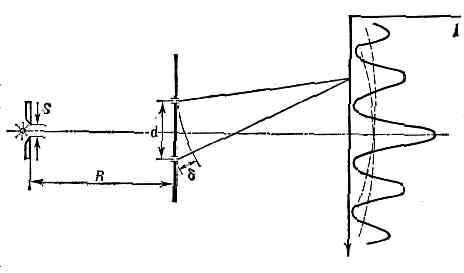
\includegraphics[scale=0.4]{figs/3_1}
  \label{fig:3_1}
\end{figure}

$$
\lambdabar_{\text{д.б.}} = \frac{\hbar}{p} \lesssim d
$$

\begin{equation}
\label{eq:3_1_1}
\Psi(\vr, t) = \brs{\psi_{1}(\vr_1) + \psi_{2}(\vr_2)} e^{-i E t /\hbar}
\end{equation}

$$
\frac{E}{\hbar} = \omega
$$

\begin{equation}
\label{eq:3_1_2}
\begin{gathered}
\abs{\Psi(\vr, t)}^2 = \abs{\psi_1(\vr_1) + \psi_2(\vr_2)}^2 = \abs{\psi_1}^2 + \abs{\psi_2}^2 + \underbrace{(\psi_1^* \psi_2 + \psi_1 \psi_2^*)}_{2 \Re(\psi_1 \psi_2^*)} = \\ = \abs{\psi_1}^2 + \abs{\psi_2}^2 + 2\abs{\psi_1}\abs{\psi_2} \cos{(\phi_1 - \phi_2)}
\end{gathered}
\end{equation}

$$
\Delta \phi = \phi_1 - \phi_2 ~~~~~~ \abs{\psi_1} = \abs{\psi_2}
$$

\begin{equation}
\label{eq:3_1_3}
\abs{\Psi}^2 = 4 \abs{\psi_1}^2 \cos^2{\frac{\Delta \phi}{2}}
\end{equation}

При этом $\abs{\Psi}^2_{max} = 4 \abs{\psi_1}^2$

Свойство \textbf{линейности} пространства состояний:
\begin{equation}
\label{eq:3_1_4}
\ket{\psi} = c_1\ket{\psi_1} + c_2\ket{\psi_2}, ~~\text{~где~} c_1, c_2 \in  \mathbb{C}
\end{equation}

\begin{stmt}[Первый постулат квантовой механики]
Квантовое состояние системы полностьб определяется вектором состояния $\ket{\psi}$. Векторы $\ket{\psi}$ и $c\ket{\psi} ~(c \neq 0)$ определяют одно и то же состояние.
\end{stmt}

Свойства пространства состояний:
\begin{enumerate}
\item $\ket{\psi} + \ket{\phi} = \ket{\phi} + \ket{\psi}$ (аксиома коммутативности)
\item $\brs{\ket{\psi} + \ket{\phi}} + \ket{\chi} = \ket{\psi} + \brs{\ket{\phi} + \ket{\chi}}$ (аксиома ассоциативности)
\item $c\brc{\ket{\phi} + \ket{\psi}} = c\ket{\phi} + c\ket{\psi}$ (аксиома дистрибутивности)
\item $(c_1 + c_2)\ket{\psi} = c_1\ket{\psi} + c_2\ket{\psi}$ (аксиома дистрибутивности)
\item $0 \cdot \ket{\psi} \equiv \ket{0} = 0$ (отсутствие квантового объекта)
\end{enumerate}

Векторное пространство состояний наделено скалярным произведением:
$$
\bk{\phi}{\psi} \in \mathbb{C}
$$

\begin{defn}
Пусть $\vec{q} = (q_1, ..., q_n)$ -- конфигурационное пространство. Тогда скалярное произведение определяется следующим образом:
\begin{equation}
\label{eq:3_1_5}
\bk{\phi}{\psi} = \int \phi^*\underbrace{(q_1, ..., q_n)}_{\vec{q}} \psi\underbrace{(q_1, ..., q_n)}_{\vec{q}} \underbrace{d q_1 ... d q_n}_{d\vec{q}}
\end{equation}
\end{defn}

Если $\bk{\phi}{\psi} = 0$, то $\phi$ и $\psi$ \textbf{взаимно ортогональны}.

Свойства скалярного произведения:
\begin{enumerate}
\item Из \eqref{eq:3_1_5}: $\bk{\phi}{\psi} = \bk{\psi}{\phi}^*$
\item Если $\ket{\tilde{\phi}} = \lambda_1\ket{\phi}$ и $\ket{\tilde{\psi}} = \lambda_2\ket{\psi}$, то $\bk{\tilde{\phi}}{\tilde{\psi}} = \lambda_1^* \lambda_2 \bk{\phi}{\psi}$
\item
	\begin{itemize}
		\item $\bk{\psi}{\psi} \geqslant 0$
		\item $\bk{\psi}{\psi} = 0 ~\Leftrightarrow~ \ket{\psi} = 0$
		\item $\norm{\psi} = \sqrt{\bk{\psi}{\psi}}$
	\end{itemize}
\end{enumerate}

Пространство состояний линейное, на нем определено скалярное произведение, и оно обладает свойством полноты, а значит является \textbf{пространством Гильберта} (обозначается буквой $\mathbb{H}$)

$\ket{\psi}$ можно понимать как столбец: $\vec{\psi} = \left(\begin{array}{c} \psi_1 \\ \psi_2 \end{array}\right)$

$$
\bk{\phi}{\psi} = (\phi_1^*, \phi_2^*) \left(\begin{array}{c} \psi_1 \\ \psi_2 \end{array}\right) = \phi_1^*\psi_1 + \phi_2^* \psi_2
$$

Т.е. состоянию $\ket{\psi}$ соответствует элемент дуального (сопряжённого) по отношению к $\mathbb{H}$ пространства $\mathbb{H}^*$, обозначаемый как $\bra{\psi}$ (или в виде строки: $(\psi_1^*, \psi_2^*)$).

Сопряжённые состояния связаны операцией \textbf{эрмитового сопряжения}, обозначаемой символом $^\dag$. На матричном языке эта операция состоит в выполнении транспонирования и комплексного сопряжения.
$$
\bra{\psi} = \ket{\psi}^\dag
$$

$$
\forall \ket{\psi} \in \mathbb{H}~~ \exists \bra{\phi} \in \mathbb{H}^* : \bk{\phi}{\psi} \in \mathbb{C}
$$

\noindent
$\ket{\psi}$ -- \textbf{кет-вектор} \\
$\bra{\psi}$ -- \textbf{бра-вектор}

Из \eqref{eq:3_1_4}:
$$
\begin{gathered}
\ket{\psi} = c_1 \ket{\psi_1} + c_2 \ket{\psi_2} \\
\bra{\psi} = c_1^* \bra{\psi_1} + c_2^* \bra{\psi_2}
\end{gathered}
$$

Нормировка:
$$
\begin{gathered}
\bk{\psi}{\psi} = \bk{\psi_1}{\psi_1} = \bk{\psi_2}{\psi_2} = 1 \\
\bk{\psi}{\psi} = \abs{c_1}^2 + \abs{c_2}^2 + 2 \Re{c_1^* c_2 \bk{\psi_1}{\psi_2}} = 1
\end{gathered}
$$

Если $\bk{\psi_1}{\psi_2} = 0$ (ортогональные состояния), то $\abs{c_1}^2 + \abs{c_2}^2 = 1$.

Вероятностная интерпретация: $\abs{c_1}^2$ ($\abs{c_2}^2$) -- вероятность обнаружить систему в состоянии \circled{1} (в состоянии \circled{2})

\begin{stmt}[Второй постулат квантовой механики]
Если измерение в состоянии \circled{1} даёт результат \circled{1}, а измерение в состоянии \circled{2} даёт результат \circled{2}, то измерение в суперпозиции этих состояний даёт либо результат \circled{1}, либо результат \circled{2}.
\end{stmt}

\section{Наблюдаемые и операторы физических величин. Линейные и эрмитовые операторы}

$F$ -- физическая (или, в терминологии Дирака, \textbf{наблюдаемая}) величина.

$F$ соответствует $\op{F}$:

$$
\begin{gathered}
\op{F}: D_{\op{F}} \to R_{\op{F}} \\
\ket{\phi} = \op{F} \ket{\psi} \in R_{\op{F}}, ~~\text{где}~~ \ket{\phi} \in D_{\op{F}}
\end{gathered}
$$

\begin{defn}
Оператор $\op{F}$ называется \textbf{линейным}, если для него выполняется:
\begin{equation}
\label{eq:3_2_1}
	\begin{gathered}
	\op{F}(c_1 \ket{\psi_1} + c_2 \ket{\psi_2}) = c_1 \op{F}\ket{\psi_1} + c_2 \op{F}\ket{\psi_2}, \\
	\text{где}~ \ket{\psi_1}, \ket{\psi_2} \in D_{\op{F}}~;~ c_1, c_2 \in \mathbb{C}\\
	\end{gathered}
\end{equation}
В этом случае:\footnote{проверить определение, просто на всякий случай}
$$
c_1 \ket{\psi_1} + c_2\ket{\psi_2} \xrightarrow{~~\op{F}~~} c_1 \ket{\phi_1} + c_2 \ket{\phi_2}
$$
\end{defn}

Алгебра линейных операторов:
\begin{enumerate}
\item Умножение на комплексное число:
$$
(c\op{F}) \ket{\psi} \equiv \underbrace{\left. c (\op{F} \ket{\psi}) \right|_{\text{\eqref{eq:3_2_1}}} = \op{F} (c \ket{\psi})}_{\text{свойство однородности $\op{F}$}}
$$
\item Коммутативность операции сложения:
$$
\begin{gathered}
(\op{F} + \op{G})\ket{\psi} \equiv \left. \op{F}\ket{\psi} + \op{G}\ket{\psi} \right|_{\text{из 1.}} = \op{G}\ket{\psi} + \op{F}\ket{\psi} = (\op{G} + \op{F})\ket{\psi}
\Rightarrow~ \op{F} + \op{G} = \op{G} + \op{F}
\end{gathered}
$$
\item Произведение операторов:
$$
\begin{gathered}
\op{P} = \op{F}\op{G} ~~\Rightarrow~~ \op{P}\ket{\psi} = \op{F}(\op{G}\ket{\psi})
\end{gathered}
$$
В общем случае операция произведения некоммутативна: $\op{F}\op{G}\ket{\psi} \neq \op{G}\op{F}\ket{\psi}$
\end{enumerate}

\begin{defn}
Выражение $\op{F}\op{G} - \op{G}\op{F}$ называется \textbf{коммутатором} операторов $\op{F}$ и $\op{G}$ и обозначается квадратными скобками:
\begin{equation}
\label{eq:3_2_2}
\brs{\op{F}, \op{G}} \equiv \op{F}\op{G} - \op{G}\op{F}
\end{equation}
Говорят, что операторы \textbf{коммутируют}, если $\brs{\op{F}, \op{G}} = 0$.
\end{defn}

Свойства коммутаторов:
\begin{enumerate}
\item Любой оператор коммутирует с константой:
$$
\brs{\op{F}, c} = 0,~~ c = \const
$$
\item Если между двумя пространствами состояний есть взаимно-однозначное соответствие, т.е.:
$$
\ket{\phi} = \op{F}\ket{\psi} ~~\to~~ \ket{\psi} = \op{G}\ket{\phi}
$$
то $\op{F}$ и $\op{G}$ являются \textbf{обратными друг к другу операторами}:
\begin{equation}
\label{eq:3_2_3}
\op{F}\op{G} = \op{G}\op{F} = 1
\end{equation}
Оператор, обратный к данному обозначается $\op{F}^{-1}$.
\end{enumerate}

\begin{equation}
\label{eq:3_2_3_add}
\op{F}\op{F}^{-1} = \op{F}^{-1}\op{F} = 1
\tag{\ref{eq:3_2_3}$'$}
\end{equation}

Обратный оператор произведения:
\begin{equation}
\label{eq:3_2_4}
(\op{F}\op{G})^{-1} = \op{G}^{-1} \op{F}^{-1}
\end{equation}

\begin{excr}
Доказать \eqref{eq:3_2_4}, используя \eqref{eq:3_2_3_add}.
\end{excr}

Рассмотрим действие $\op{F}$ в гильбертовом пространстве $\mathbb{H}$ (и, соответственно, оператора $\op{F}^\dag$ в $\mathbb{H}^*$):

$$
\ket{\chi} = \op{F}\ket{\psi} ~\to~ \ket{\chi}^\dag = \left. (\op{F}\ket{\psi})^\dag \right|_{(\op{A}\op{B})^\dag = \op{B}^\dag \op{A}^\dag} = \bra{\psi} \op{F}^\dag
$$

\begin{equation}
\label{eq:3_2_5}
\boxed{
	\bra{\chi} = \bra{\psi} \op{F}^\dag
}
\end{equation}

Из \eqref{eq:3_2_5}:
$$
\bk{\chi}{\phi} = \bfk{\psi}{\op{F}^\dag}{\phi} = \bk{\phi}{\chi}^* = \bfk{\phi}{\op{F}}{\psi}^*
$$

\begin{defn}
Эрмитово-сопряжённым к $\op{F}$ называется следующий оператор:
\begin{equation}
\label{eq:3_2_6}
\boxed{
	\bfk{\psi}{\op{F}^\dag}{\phi} = \bfk{\phi}{\op{F}}{\psi}^*
}
\end{equation}
\end{defn}

Свойства эрмитово-сопряжённых операторов:
\begin{itemize}
\item $(c\op{F})^\dag = c^* \op{F}^\dag$
\item $(\op{F}^\dag)^\dag = \op{F}$
\item $(\op{F} + \op{G})^\dag = \op{F}^\dag + \op{G}^\dag$
\item $(\op{F}\op{G})^\dag = \op{G}^\dag \op{F}^\dag$
\end{itemize}

\begin{excr}
Доказать приведённые выше свойства.
\end{excr}

\begin{defn}
Если $\op{F}^\dag = \op{F}$ или выполняется следующее равенство:
\begin{equation}
\label{eq:3_2_7}
\forall \ket{\psi},\ket{\phi} \in D_{\op{F}} ~~\to~~  \bk{\psi}{\op{F}\psi} = \bfk{\phi}{\op{F}}{\psi}^*
\end{equation}
то оператор $\op{F}$ называется \textbf{эрмитовым} или \textbf{самосопряжённым}.
\end{defn}

Для состояний $\ket{\psi}$ и $\ket{\phi}$:
$$
\op{F}\ket{\psi} \equiv \ket{\op{F}\psi}
$$

Альтернативное определение эрмитового сопряжения: $\op{F}^\dag$ эрмитово-сопряжённый, если:
\begin{equation}
\label{eq:3_2_6_add}
\boxed{
	\bk{\phi}{\op{F}\psi} = \bk{\op{F}^\dag\phi}{\psi}
} = \bk{\psi}{\op{F}^\dag \phi}^*
\tag{\ref{eq:3_2_6}$'$}
\end{equation}
или
\begin{equation}
\label{eq:3_2_6_add_x2}
\boxed{
	\bk{\psi}{\op{F}^\dag \phi} = \bk{\op{F} \psi}{\phi}
}
\tag{\ref{eq:3_2_6}$''$}
\end{equation}
что эквивалентно:
$$
\int \psi^*(\vec{q}) \op{F}^\dag \phi(\vec{q}) d\vec{q} = \int \brc{\op{F} \psi(\vec{q})}^* \phi(\vec{q}) d\vec{q}
$$

\begin{defn}
$\op{F}$ называется \textbf{эрмитовым} (самосопряжённым), если $\op{F}^\dag = \op{F}$, т.е.:
\begin{equation}
\label{eq:3_2_7_add}
\forall \ket{\psi}, \ket{\phi} \in D_{\op{F}}  ~\to~ \boxed{ \bk{\psi}{\op{F} \phi} = \bk{\op{F}\psi}{\phi} }
\tag{\ref{eq:3_2_7}$'$}
\end{equation}
или
$$
\int \psi^*(\vec{q}) \op{F} \phi(\vec{q}) d\vec{q} = \int \brc{\op{F} \psi(\vec{q})}^* \phi(\vec{q}) d\vec{q}
$$
\end{defn}

Замечание:
\begin{enumerate}
\item $\norm{\psi} < \infty$, $\norm{\phi} < \infty$
\item $\norm{\op{F} \psi} < \infty$, $\norm{\op{F} \phi} < \infty$
\end{enumerate}

\begin{defn}
Выражение:
$$
\bk{\phi}{\op{F}\psi} \equiv \bfk{\phi}{\op{F}}{\psi} = \int \phi^*(\vec{q})\op{F}\psi(\vec{q}) d\vec{q}
$$
называется \textbf{матричным элементом} оператора $\op{F}$ на функциях $\phi$ и $\psi$, или матричным элементом $\op{F}$ \textbf{в обкладках} $\bra{\phi}$ и $\ket{\psi}$  

Величина $\bk{\psi}{\op{F}\psi} \equiv \bfk{\psi}{\op{F}}{\psi}$ называется \textbf{диагональным матричным элементом}.
\end{defn}

Из \eqref{eq:2_2_1}, среднее значение физической величины:
\begin{equation}
\label{eq:3_2_8}
\boxed {
	\avg{F} = \bk{\psi}{\op{F}\psi} = \bfk{\psi}{\op{F}}{\psi}
}
\end{equation}

Для величины, принимающей действительные значения, $\avg{F} = \avg{F}^*$.

Из \eqref{eq:3_2_8}:
\begin{equation}
\label{eq:3_2_9}
\bfk{\psi}{\op{F}}{\psi} = \left .\bfk{\psi}{\op{F}}{\psi}^* \right|_{\text{\eqref{eq:3_2_6}}} = \bfk{\psi}{\op{F}^\dag}{\psi}
\end{equation}

Следовательно: $\op{F} = \op{F}^\dag$.

Таким образом, физическим (наблюдаемым) величинам соответствуют \textbf{эрмитовы операторы}.

Рассмотрим среднеквадратичное отклонение (дисперсию):
\begin{equation}
\label{eq:3_2_10}
\avg{(\Delta F)^2} \equiv \avg{(F - \avg{F}^2)}
\end{equation}

Из \eqref{eq:2_2_1}:
\begin{equation}
\label{eq:3_2_11}
\avg{(\Delta F)^2} = \bfk{\psi}{(\op{F} - \avg{F})^2}{\psi}
\end{equation}

Заметим, что $\op{F} - \avg{F}$ -- эрмитов оператор.

\begin{equation}
\label{eq:3_2_12}
\left. \avg{(\Delta F)^2} \right|_{\text{\eqref{eq:3_2_7_add}}} = \bk{(F - \avg{F})\psi}{(F - \avg{F})\psi} = \int \abs{\brc{F - \avg{F}}\psi}^2 d\vec{q} \geqslant 0
\end{equation}

Если $\avg{(\Delta F)^2} = 0$, т.е. величина не имеет разброса, то из \S 3 гл. 2:
\begin{equation}
\label{eq:3_2_13}
\op{F}\ket{\psi} = \avg{F}\ket{\psi}
\end{equation}

Примем $\avg{F} = f$ -- собственное значение оператора $\op{F}$.

Можно переписать формулу \eqref{eq:2_3_2}:
\begin{equation}
\label{eq:3_2_14}
\op{F}\ket{\psi_{f}} = f \ket{\psi_{f}}
\end{equation}

\begin{stmt}[Третий постулат квантовой механики]
Физическая величина $F$ в любом квантовом состоянии может принимать только те значения, которые принадлежат спектру её оператора $\op{F}$.
\end{stmt}

\begin{thm}
Если оператор $\op{F}$ эрмитов, то он имеет вещественные собственные значения.
\end{thm}
\begin{proof}
Левая часть \eqref{eq:3_2_14}:
$$
\left. \bfk{\psi_f}{\op{F}}{\psi_f}^* \right|_{\text{\eqref{eq:3_2_7}}} = \bfk{\psi_f}{\op{F}}{\psi_f}
$$
Правая часть \eqref{eq:3_2_14}:
$$
f^*\bk{\psi_f}{\psi_f}^* = f^* \bk{\psi_f}{\psi_f} = f\bk{\psi_f}{\psi_f}
$$
Следовательно $\boxed{f^* = f}$.
\end{proof}

\begin{stmt}
Эрмитовы операторы изображают вещественные (наблюдаемые) величины.
\end{stmt}

\section{Условие ортогональности и полноты для собственных функций операторов физических величин}

Уравнение \eqref{eq:2_3_3} на собственные значения $\op{F}$ в векторном виде:

\begin{equation}
\label{eq:3_3_1}
\op{F}\ket{\psi_n} = f_n \ket{\psi_n} ~~\text{или}~~ \op{F}\ket{n} = f_n\ket{n}
\end{equation}
где $\psi_n \equiv \ket{n}$, $n = 0, 1, 2, ...$

\noindent
$f_n \to \ket{\psi_n}$ -- невырожденный (простой) спектр\\
$f_n \to \brcr{\ket{\psi_n^{(1)}}, \ket{\psi_n^{(2)}}, ..., \ket{\psi_n^{(g)}} }$ -- вырожденный спектр

\begin{defn}
Максимальное количество линейно-независимых собственных векторов (собственных функций), отвечающих данному собственному значению, называется \textbf{кратностью вырождения} этого собственного значения.
\end{defn}

\begin{stmt}
Собственные векторы эрмитового оператора, соответствующие различным собственные значениям, взаимно ортогональны.
\end{stmt}
\begin{proof}

\begin{equation}
\label{eq:3_3_2}
	\begin{gathered}
		\bra{\psi_m}: \op{F}\ket{\psi_n} = f_n \ket{\psi_n} \\
		\bra{\psi_n}: \op{F}\ket{\psi_m} = f_m \ket{\psi_m} \\
		f_n \neq f_m
	\end{gathered}
\end{equation}

$$
\left. \bfk{\psi_m}{\op{F}}{\psi_n} - \bfk{\psi_n}{\op{F}}{\psi_m}^\dag \right|_{\text{\eqref{eq:3_2_7}}} = 0 = f_n \bk{\psi_m}{\psi_n} - \underbrace{f_m^*}_{= f_m} \bk{\psi_n}{\psi_m}^*
$$

\begin{equation}
\label{eq:3_3_3}
(f_n - f_m) \bk{\psi_m}{\psi_n} = 0
\end{equation}

$f_m \neq f_n ~~\to~~ \boxed{\bk{\psi_m}{\psi_n} = 0}$

\end{proof}

\begin{equation}
\label{eq:3_3_4}
\bk{\psi_n}{\psi_n} = 1
\end{equation}

Из \eqref{eq:3_3_3} и \eqref{eq:3_3_4} получим условие ортонормированности:
\begin{equation}
\label{eq:3_3_5}
\boxed{
	\bk{\psi_m}{\psi_n} = \bk{m}{n} = \delta_{mn}
}
\end{equation}

$$
f_n ~\to~ \brcr{\ket{\psi_n^{(i)}}} ~~ i = \overline{1,g}
$$

\begin{equation}
\label{eq:3_3_6}
f_n ~\to~ \ket{\psi_n^s} = \sum_{i=1}^{g} c_i^{(s)} \ket{\psi_n^{(i)}}
\end{equation}

Посредством ортогонализации методом Грамма-Шмидта, коэффициенты $c_i^{(s)}$ возможно подобрать так, что $\bk{\psi_n^{(t)}}{\psi_n^{(s)}} = \delta_{ts}$

Ортонормированная система -- базис в гильбертовом пространстве состояний.

\begin{equation}
\label{eq:3_3_7}
\forall \ket{\psi} \in \mathbb{H} ~~~ \op{F}:~~ \ket{\psi} = \sum_n c_n \ket{\psi_n}
\end{equation}

$$
\bk{\psi_m}{\psi} = \sum_n c_n \underbrace{\bk{\psi_m}{\psi_n}}_{=\delta{mn}~(\text{из \eqref{eq:3_3_5}})} = \sum_n c_n \delta_{mn} = c_m
$$

$c_n = \bk{\psi_n}{\psi}$ -- коэффициенты -- проеции вектора на соответствеющие орты.

Для векторов-состояний $\ket{\psi}$ и $\bra{\phi}$ выполняется $\bk{\phi}{\psi} \in \mathbb{C}$

\begin{equation}
\label{eq:3_3_8}
\op{P}_{\psi} = \proj{\psi}{\phi}
\end{equation}

\begin{equation}
\label{eq:3_3_9}
\op{P}_\psi \ket{\chi} = \ket{\psi} \underbrace{\bk{\phi}{\chi}}_{= c} = c \ket{\psi}
\end{equation}

Следовательно, $\op{P}_\psi$ -- \textbf{оператор проектирования}.

Из \eqref{eq:3_3_7}:
\begin{equation}
\label{eq:3_3_10}
\ket{\psi} = \sum_n \ket{\psi_n} \bk{\psi_n}{\psi} = \brc{\sum_n \proj{\psi_n}{\psi_n}} \ket{\psi}
\end{equation}

Итого, получаем \textbf{условие полноты} (операторное разложение единицы) системы собственных векторов оператор $\op{F}$:
\begin{equation}
\label{eq:3_3_11}
\boxed {
	\sum_n \proj{\psi_n}{\psi_n} = \mathds{1}
}
\end{equation}

\begin{equation}
\label{eq:3_3_12}
\ket{\psi_n} \underbrace{\bk{\psi_n}{\psi}}_{ = c_n} \equiv \op{P}_n \ket{\psi} = c_n \ket{\psi_n}
\end{equation}
где $\proj{\psi_n}{\psi_n} = \op{P}_n$ -- проектор на n-е базисное состояние.

\noindent
Свойства проекторов:
\begin{enumerate}
\item $\op{P}_n$ -- эрмитов
\item $\op{P}_n^2 = \op{P}_n$
\item собственные значения $\op{P}_n$: $\lambda = \brcr{0, 1}$
\end{enumerate}
\begin{excr}
Доказать вышеперечисленные свойства.
\end{excr}

$$
\begin{gathered}
\left. \ket{\psi} \right|_{\text{\eqref{eq:3_3_7}}} = \sum_n c_n \ket{\psi_n} \\
\bra{\psi} = \sum_m c_m^* \bra{\psi_m}
\end{gathered}
$$

\begin{equation}
\label{eq:3_3_13}
\bk{\psi}{\psi} = \sum_m \sum_n c_m^* c_n \underbrace{\bk{\psi_m}{\psi_n}}_{\delta_{mn}} = \boxed{\sum_n \abs{c_n}^2 = 1}
\end{equation}

Подставляя \eqref{eq:3_3_7} в \eqref{eq:3_2_8}:
\begin{equation}
\label{eq:3_3_14}
	\begin{gathered}
		\avg{F} = \bfk{\psi}{\op{F}}{\psi} = \sum_m \sum_n c_m^* c_n \underbrace{ \bfk{\psi_m}{F}{\psi_n} }_{\bfk{\psi_m}{f_n}{\psi_n}~\text{из \eqref{eq:3_3_1}}} =
		\sum_m \sum_n c_m^* c_n f_n \underbrace{\bk{\psi_m}{\psi_n}}_{\delta{mn}} = \\ = \boxed{\sum_n f_n \abs{c_n}^2 = \avg{F}}
	\end{gathered}
\end{equation}

$\abs{c_n}^2 = \abs{\bk{\psi_n}{\psi}}^2$ -- вероятность обнаружить $F = f_n$ при измерении.

При большом количестве измерений:
$$
\boxed {
	P_{\ket{\psi}}(F = f_n) = \abs{\bk{\psi_n}{\psi}}^2
}
$$

$$
P_{\ket{\psi}}(F = f_n) = \bra{\psi} \underbrace{\psi_n \rangle \langle \psi_n}_{\op{P}_n} \ket{\psi} \equiv \avg{\op{P}_n}_{\ket{\psi}}
$$

\section{Нормировка собственных функций на единицу и дельта-функцию}

\textbf{Пример непрерывного спектра:}

Из \eqref{eq:2_3_1}:
\begin{equation}
\label{eq:3_4_1}
\op{\vp} \Psi_{\vp}(\vr, t) = \vp \Psi_{\vp}(\vr, t),
\end{equation}
где $\Psi_{\vp}(\vr, t) = \frac{1}{(2\pi \hbar)^{3/2}} e^{(i/\hbar) (\vp \vr - Et)}$ (\eqref{eq:2_1_2})

\begin{equation}
\label{eq:3_4_2}
\int \Psi_{\vp'}(\vr, t) \Psi_{\vp}(\vr, t) dv \equiv \bk{\vp'}{\vp} = \delta(\vp - \vp')
\end{equation}

Введём \textbf{оснащённое} гильбертово пространство (имеющее обобщённые собственные векторы).
\begin{equation}
\label{eq:3_4_3}
\boxed {
	\op{F} \ket{f} = f\ket{f}, ~~\text{где}~ \bk{f}{f'} = \delta(f-f')
}
\end{equation}
где $\ket{f}$ -- векторы непрерывного спектра.

\begin{thm}
Самосопряжённый оператор обладает в оснащённом гильбертовом пространство \textbf{полной} системой обобщённых собственных векторов, отвечающих вещественным собственным значениям.
\end{thm}

Рассмотрим возможные варианты спектра:
\begin{enumerate}
\item $\op{F}$ имеет дискретный спектр
\begin{equation}
\label{eq:3_4_4}
\left. \ket{\psi} \right|_{\text{\eqref{eq:3_3_7}}} = \sum_n c_n \ket{\psi_n} \equiv \sum_n c_n \ket{n}
\end{equation}

\item $\op{F}$ имеет непрерывный спектр
\begin{equation}
\label{eq:3_4_5}
\ket{\psi} = \int c(f) \ket{f} df
\end{equation}
где $c_n \bk{\psi_n}{\psi} \equiv \bk{n}{\psi}$

$$
\bk{f'}{\psi} = \int c(f) \underbrace{\bk{f'}{f}}_{\delta(f-f')~\text{из \eqref{eq:3_4_3}}} df = c(f')
$$
или
$$
\boxed {
	c(f) = \bk{f}{\psi}
}
$$

\item $\op{F}$ имеет смешанный спектр (задача 5 из 1-го задания)
\begin{equation}
\label{eq:3_4_6}
\boxed {
	\ket{\psi} = \sum_n \ket{n}\bk{n}{\psi} + \int df \ket{f} \bk{f}{\psi}
}
\end{equation}
-- разложение произвольного $\ket{\psi}$ по \textbf{полному} базису оператора $\op{F}$.
\end{enumerate}

Из \eqref{eq:3_4_5}:
$$
\ket{\psi} = \int \bk{f}{\psi} \cdot \ket{f} df = \int df \cdot \ket{f} \bk{f}{\psi}
$$

Отсюда получаем условие полноты в непрерывном спектре:
$$
\boxed {
	\int df \proj{f}{f} = \mathds{1}
}
$$

Обобщённое словие полноты:
\begin{equation}
\label{eq:3_4_7}
\boxed {
	\sum_n \proj{n}{n} + \int df \proj{f}{f} = \mathds{1}
}
\end{equation}

Рассмотрим физический смысл $c_n = \bk{n}{\psi}$ и $c(f) = \bk{f}{\psi}$ в разложении \eqref{eq:3_4_6}.

Обобщённые условия ортонормировки (из \eqref{eq:3_3_5} и \eqref{eq:3_4_3}):
$$
\bk{n}{m} = \delta_{nm}, ~~~~ \bk{f}{f'} = \delta(f - f') ~~~~ \bk{n}{f} = 0
$$

Из \eqref{eq:3_4_6}:
\begin{equation}
\label{eq:3_4_8}
\boxed {
	\bk{\psi}{\psi} = \sum_n \abs{c_n}^2 + \int \abs{c(f)}^2 df = 1
}
\end{equation}

\begin{excr}
Доказать \eqref{eq:3_4_8}.
\end{excr}

Подставляя \eqref{eq:3_4_8} в \eqref{eq:3_2_8} и используя задачи на собственные значения \eqref{eq:3_3_1} и \eqref{eq:3_4_3}, получим:
\begin{equation}
\label{eq:3_4_9}
\boxed {
	\avg{F} = \bfk{\psi}{\op{F}}{\psi} = \sum_n f_n \abs{c_n}^2 + \int f \underbrace{\abs{c(f)}^2 df}_{dp}
}
\end{equation}

Из \eqref{eq:3_4_8} и \eqref{eq:3_4_9} следует, что $\abs{c_n}^2 = \abs{\bk{n}{\psi}}^2$ -- вероятность того, что при измерении физической величины $F$ в состоянии $\ket{\psi}$ будет получено $F = f_n$. \footnote{см. пар.3, 3 том Ландау-Лившица}

Если $f_n$ -- вырожденное собственное значение, такое, что кратность его вырождения равна $g$, то:
\begin{equation}
\label{eq:3_4_10}
P_{\ket{\psi}}(F = f_n) = \sum_{i=1}^{g} \abs{c_n^{(i)}}^2 \equiv \sum_{i=1}^{g} \abs{ \bk{n^{(i)}}{\psi} }^2
\end{equation}

Плотность вероятности получить значение, лежащее в окрестности $(f, f + df)$ точке непрерывного спектра $f$ равна:

\begin{equation}
\label{eq:3_4_11}
\boxed {
	\rho_{\ket{\psi}}(f) = \D{P}{f} = \abs{c(f)}^2
} = \abs{\bk{f}{\psi}}^2
>>>>>>> Добавлены изменения Елены Лимоновой
\end{equation}